\documentclass{beamer}
\usepackage{multirow}
\usepackage{tikz}
\usetikzlibrary{calc}
\usetikzlibrary{decorations.pathreplacing}
\usetikzlibrary{matrix,shapes.geometric}
\usepackage{booktabs}
\usepackage[backend=biber,
style=authoryear-comp]{biblatex}

\setbeamercovered{transparent}
\usetheme{Madrid}
\bibliography{sample.bib}

\title{Systemic Risk and Financial Connectedness: Empirical Evidence}
\author{Mateusz Dadej}
\institute{Phd. student at Universita degli Studi di Brescia, ITA \\
Visiting researcher at Universität Mannheim, DE}
\date{Forecasting Financial Markets Conference 2024
\\
Worcester College, University of Oxford}

% Removes icon in bibliography
\setbeamertemplate{bibliography item}{}

\begin{document}

\titlepage


\begin{frame}{Theoretical background}   
\begin{itemize}
    \item<1-> "Robust-yet-fragile" property of financial system can serve at the same time as shock-absorbers and shock-amplifiers to the financial sector (\cite{haldane}).
    \item<2-> This makes the system robust, when the magnitude of shock is relatively small, but fragile, when the shock is large. 
    \item<3-> A seminal paper by \cite{acemoglu}, provides a formal model, in which an extent of financial contagion exhibits a form of regime transition.
    \begin{itemize}
      \item<4-> When the shocks are small, the damages are dissipated through large number of financial institutions.
      \item<5-> When the shock is above some threshold, the properties of the system changes markedly. The damages are amplified through the network.
    \end{itemize}
  \end{itemize}
\end{frame}


\begin{frame}{Research design}
\begin{itemize}
    \item<1->The aim is to provide (and quantify) empirical evidence for the regime-dependent effect of connectedness on financial stability, i.e.:
    \begin{itemize}
        \item<2-> Stable markets regime: Higher connectedness $\rightarrow$ less volatility
        \item<3-> High shock regime: Higher connectedness $\rightarrow$ more volatility
    \end{itemize}
    \,
    \item<4-> In a following steps:
    \begin{itemize}
        \item<5-> Based on stock prices of the biggest banks in EU and USA, I calculate the connectedness measures in a rolling window basis.
        \item<6-> This time series measure is then used as an explanatory variable in a Markov switching ARCH model.    
    \end{itemize}
\end{itemize}

\end{frame}    

\begin{frame}{(Financial) network estimation from time series}
\scalebox{0.75}{\begin{minipage}{1.2\textwidth}
		
	\begin{figure}
		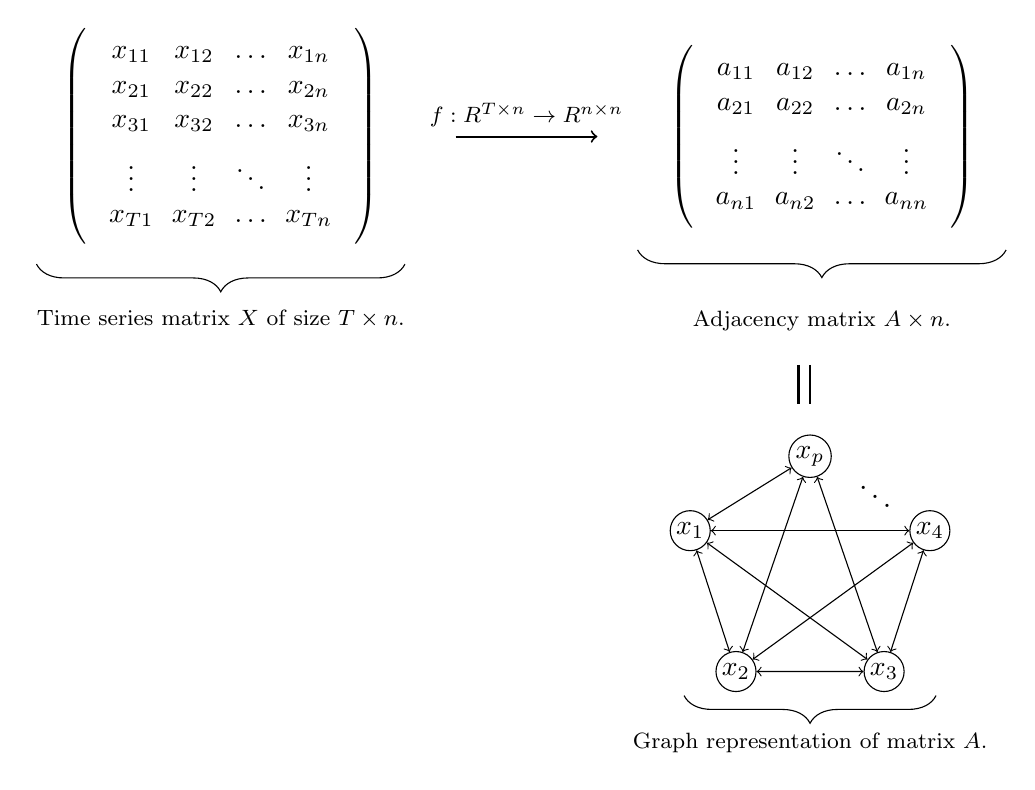
\begin{tikzpicture}	
			% Matrix
			\begin{scope}[scale = 0.9, xshift=0.5]
				\matrix (m) [matrix of math nodes,left delimiter=(,right delimiter=),ampersand replacement=\&] {
					x_{11} \& x_{12} \& \dots \& x_{1n} \\
					x_{21} \& x_{22} \& \dots \& x_{2n} \\
					x_{31} \& x_{32} \& \dots \& x_{3n} \\
					\vdots \& \vdots \& \ddots \& \vdots \\
					x_{T1} \& x_{T2} \& \dots \& x_{Tn} \\
				};
				
				\draw [decorate,decoration={brace,amplitude=10pt}]
				(2.6,-1.8) -- (-2.6,-1.8) node [black,midway,xshift=0cm,yshift=-0.7cm] 
				{\footnotesize Time series matrix $\boldsymbol{X}$ of size $T \times n$.};
			\end{scope}
			
			\begin{scope}[scale= 0.6]
				\draw[->, line width = 0.7] (5,0) -- (8,0) node[midway, above] {\footnotesize $f: \mathbb{R}^{T\times n}\to \mathbb{R}^{n \times n}$};
			\end{scope}
			
			\begin{scope}[scale = 0.9, xshift = 8.5cm]
				\matrix (m) [matrix of math nodes,left delimiter=(,right delimiter=),ampersand replacement=\&] {
					a_{11} \& a_{12} \& \dots \& a_{1n} \\
					a_{21} \& a_{22} \& \dots \& a_{2n} \\
					\vdots \& \vdots \& \ddots \& \vdots \\
					a_{n1} \& a_{n2} \& \dots \& a_{nn} \\
				};
				
				\draw[decorate,decoration={brace,amplitude=10pt}]
				(2.6,-1.6) -- (-2.6,-1.6) node [black,midway,yshift=-0.9cm] 
				{\footnotesize Adjacency matrix $\boldsymbol{A} \times n$.};
			\end{scope}
			
			\draw[line width=1pt] (7.5,-2.9) -- (7.5,-3.4);
			\draw[line width=1pt] (7.35,-2.9) -- (7.35,-3.4);
			
			% Pentagram graph
			\begin{scope}[xshift=7.5cm, yshift = -5.5cm, scale=0.8]
				\node[draw, circle, inner sep=1pt] (a) at (90:1.8) {$x_p$};
				\node[draw, circle, inner sep=1pt] (b) at (162:2) {$x_1$};
				\node[draw, circle, inner sep=1pt] (c) at (234:2) {$x_2$};
				\node[draw, circle, inner sep=1pt] (d) at (306:2) {$x_3$};
				\node[draw, circle, inner sep=1pt] (e) at (18:2) {$x_4$};
				
				\draw[<->] (a) -- (c);
				\draw[<->] (c) -- (e);
				\draw[<->] (e) -- (b);
				\draw[<->] (b) -- (d);
				\draw[<->] (d) -- (a);
				
				\draw[<->] (a) -- (b);
				\draw[<->] (b) -- (c);
				\draw[<->] (c) -- (d);
				\draw[<->] (d) -- (e);
				\node[xshift=1.9, yshift=2.1, scale=1.1] at ($(e)!.5!(a)$) {$\ddots$};
				%\draw[dotted, <->] (e) -- (a);
				
				\draw [decorate,decoration={brace,amplitude=10pt}]
				(2,-2) -- (-2,-2) node [black,midway, yshift=-0.6cm] 
				{\footnotesize Graph representation of matrix $\boldsymbol{A}$.};
				
			\end{scope}
		\end{tikzpicture}
	\end{figure}
	
		
\end{minipage}}
\end{frame}

\begin{frame}{Connectedness measures - denoted $\kappa_t$}

\begin{enumerate}
    \item<1-> Average correlation: $\frac{\sum_{i \neq i}^{N} \sum_{j \neq j}^{N} \rho_{i,j}(R)}{N^2-N}$,  with $\rho(\cdot)$ being the Ledoit-Wolf estimator of the covariance matrix (\cite{ledoit}).
    \item<2-> $\frac{\sum_{i}^{k} \lambda_i}{\sum_{i}^{N} \lambda_i}$, with $\lambda$ being an eigenvalue of the covariance matrix. 
    \item<3-> (\cite{granger}) - based measure of connectedness:
    \begin{itemize}
        \item<4-> For each of stock pair estimate: $r_{i,t+1} = \beta_0 + \beta_1 r_{m, t} + \beta_2 r_{j, t} + \sum_{k}^{s} \beta_{c+2} x_{c, t} + \epsilon_t$
        \item<5-> The "causality" matrix is set as: $G_{i,j} = \begin{cases}
            1  & \text{if } \beta_2 \text{ is significant} \\
            0 & \text{otherwise}
          \end{cases} \forall i \neq j$
        \item<6-> As with before we calculate average connectedness: $\frac{\sum_{i \neq j}^{N} \sum_{j \neq i}^{N} G_{i,j}}{ N \times (N-1)}$
    \end{itemize}
\end{enumerate}
    (Last two measures are as described in \cite{billio})
\end{frame}

\begin{frame}{Connectedness measures results}

\begin{figure}[H]
    \caption{Standardized time series of connectedness measures for a rolling window of 63 trading days (quarter)}
    \includegraphics[scale=0.3]{connectmeasures.png}
    \centering
\end{figure}    

\end{frame}    

\begin{frame}{Modeling the regime-dependent effect of connectedness}

Mean specification of the model: 

$$r_{b,t} = \beta_0 + \underbrace{\beta_1 r_{b,t-1}}_{\text{Banking index}} + \underbrace{\beta_2 r_{m,t-1}}_{\text{Broad market index}} + \epsilon_t$$

The Markov-switching ARCH specification is:

$$\sqrt{\epsilon^2_t} = \alpha_{0,s} + \underbrace{\alpha_{1,s}\kappa_{t-1}}_{\text{connectedness}} + \underbrace{\sum_{i=1}^{p} \alpha_{i+1} \sqrt{\epsilon^2_{t-i}}}_{\text{Lag controls}}$$


With regime changes according to Markov process: \begin{equation*}
    P(S_t = i | S_{t-1} = j) = \begin{bmatrix}
      \pi_1 & 1 - \pi_2\\
        1 - \pi_1 & \pi_2
        \end{bmatrix}
\end{equation*}

\end{frame}

\begin{frame}{Estimation results}
    EU banking sector and 252 trading days (year) rolling window 
    \begin{table}\small
        \begin{tabular}{cccccc}
          \toprule
           Connectedness measure &  & \multicolumn{2}{c}{\bfseries Regime 1} & \multicolumn{2}{c}{\bfseries Regime 2}  \\
           %\cmidrule(lr){1-6}
           \hline
           & & Estimate & S.E. & Estimate & S.E. \\
           \hline
           \multirow{3}{*}[\normalbaselineskip]{Correlation-based} & $\alpha_0$ & 0.466* & 0.019 & 1.988*  & 0.06 \\
            & $\alpha_1$ & 0.017 & 0.009 & 0.22* & 0.043 \\
            & $\eta$ & 0.435 & 0.009 & 1.4 & 0.012 \\
            & $\pi_{i,i}$ &  \multicolumn{2}{c}{78.6\%} & \multicolumn{2}{c}{52\%}\\
            \hline
            \multirow{3}{*}[\normalbaselineskip]{Eigenvalue-based} & $\alpha_0$ & 0.458* & 0.018 & 1.975*  & 0.061 \\
            & $\alpha_1$ & -0.002 & 0.008 & 0.052 & 0.048 \\
            & $\eta$ & 0.435 & 0.009 & 1.42 & 0.012 \\
            & $\pi_{i,i}$ &  \multicolumn{2}{c}{90\%} & \multicolumn{2}{c}{67.2\%}\\
            \hline
            \multirow{3}{*}[\normalbaselineskip]{Granger-based} & $\alpha_0$ & 0.468* & 0.018 & 1.984*  & 0.059 \\
            & $\alpha_1$ & 0.018* & 0.008 & 0.276* & 0.05 \\
            & $\eta$ & 0.433 & 0.009 & 1.394 & 0.013 \\
            & $\pi_{i,i}$ &  \multicolumn{2}{c}{78.5\%} & \multicolumn{2}{c}{52.5\%}\\
            \hline
          \multicolumn{6}{l}{\footnotesize * coefficient with 5\% statistical significance} \\
          \hline
        \end{tabular}
      \end{table}

\end{frame}    

\begin{frame}
    US banking sector and 63 trading days (year) rolling window
    \begin{table}\small
        \begin{tabular}{cccccc}
          \toprule
           Connectedness measure &  & \multicolumn{2}{c}{\bfseries Regime 1} & \multicolumn{2}{c}{\bfseries Regime 2}  \\
           %\cmidrule(lr){1-6}
           \hline
           & & Estimate & S.E. & Estimate & S.E. \\
           \hline
           \multirow{3}{*}[\normalbaselineskip]{Correlation-based} & $\alpha_0$ & 0.402* & 0.013 & 1.517*  & 0.054 \\
            & $\alpha_1$ & 0.027* & 0.007 & 0.239* & 0.044 \\
            & $\eta$ & 0.373 & 0.007 & 1.268 & 0.017 \\
            & $\pi_{i,i}$ &  \multicolumn{2}{c}{89.4\%} & \multicolumn{2}{c}{67\%}\\
            \hline
            \multirow{3}{*}[\normalbaselineskip]{Eigenvalue-based} & $\alpha_0$ & 0.416* & 0.014 & 1.554*  & 0.057 \\
            & $\alpha_1$ & 0.041* & 0.007 & 0.194* & 0.046 \\
            & $\eta$ & 0.38 & 0.006 & 1.304 & 0.016 \\
            & $\pi_{i,i}$ &  \multicolumn{2}{c}{90\%} & \multicolumn{2}{c}{67.2\%}\\
            \hline
            \multirow{3}{*}[\normalbaselineskip]{Granger-based} & $\alpha_0$ & 0.379* & 0.013 & 1.472*  & 0.047 \\
            & $\alpha_1$ & 0.009 & 0.007 & 0.205* & 0.032 \\
            & $\eta$ & 0.356 & 0.006 & 1.161 & 0.013 \\
            & $\pi_{i,i}$ &  \multicolumn{2}{c}{87.4\%} & \multicolumn{2}{c}{65\%}\\
            \hline
          \multicolumn{6}{l}{\footnotesize * coefficient with 5\% statistical significance} \\
          \hline
        \end{tabular}
      \end{table}

\end{frame}    

\begin{frame}{Robustness check - design}
  
    \begin{itemize}
      \item<1-> Are there confounders in the bank specific characteristics?
      \item<2-> To check this I use quarterly financial statement data:
      \begin{itemize}
        \item<3-> I use financial statement data from Orbis database.
        \item<4-> Substantial reduction of used data due to lower frequency of reports and their availability.
        \item<5-> $N$ banks: $51 \rightarrow 30$. $T$ observations $6240 \rightarrow 260$.
        \item<6-> Quarterly financial data was interpolated (with splines) into weekly data.
        \item<7-> Financial ratios and financial variable growth was used as a control in the Granger-based connectedness estimation
      \end{itemize}
\end{itemize}
\end{frame}

\begin{frame}{Robustness check - results}
  Results for EU banks with a rolling window of 52 weeks
  \begin{table}\small
    \begin{tabular}{cccccc}
      \toprule
       Granger-based &  & \multicolumn{2}{c}{\bfseries Regime 1} & \multicolumn{2}{c}{\bfseries Regime 2}  \\
       %\cmidrule(lr){1-6}
       \hline
       & & Estimate & S.E. & Estimate & S.E. \\
       \hline
       \multirow{3}{*}[\normalbaselineskip]{Correlation-based} & $\alpha_0$ & 1.554* & 0.206* & 4.44*  & 0.59 \\
        & $\alpha_1$ & 0.106 & 0.108 & 0.843* & 0.45 \\
        & $\eta$ & 1.084 & 0.034 & 2.52 & 0.086 \\
        & $\pi_{i,i}$ &  \multicolumn{2}{c}{88.6\%} & \multicolumn{2}{c}{57\%}\\
        \hline
      \multicolumn{6}{l}{\footnotesize * coefficient with 5\% statistical significance} \\
      \hline
    \end{tabular}
  \end{table}
\end{frame}  


\begin{frame}{Conclusions and future research directions}
\begin{itemize}
  \item<1-> The theory is confirmed to some degree - the connectedness effect is indeed regime dependent.
  \item<2-> The effect is asymmetric - the connectedness is more important in the high shock regime.
  \item<3-> Further research 
  \begin{itemize}
    \item<4-> should control for firm specific balance sheet (preliminarily, the results hold)
    \item<5-> Possible application of Gaussian graphical models to estimate the connectedness measures
  \end{itemize}
  \item<6-> contact: m.dadej@unibs.it Thank you!
\end{itemize}
\end{frame}

\begin{frame}
	Thank you!
	
	The working paper is available at \url{m-dadej.github.io/files/connectedness.pdf}
\end{frame}


\begin{frame}[allowframebreaks]
\frametitle{References}
  \printbibliography
\end{frame}

\end{document}